\documentclass[12pt]{article} 

\usepackage[latin1]{inputenc}
\usepackage[spanish]{babel}
\usepackage{color}
\usepackage{multicol}
\usepackage{amsmath}
\usepackage{amssymb}
\usepackage{enumerate}
\usepackage{graphics}
\usepackage{graphicx}

\title{TRAIN}
\author{Sara Chica, Rodrigo Gualtero}
\date{24 de Noviembre, 2012}

\begin{document}
\maketitle
\tableofcontents

\section{Introducci�n}
Este es un problema de la UVA, identificado con el c�digo \textit{299}, en el cual se desea ordenar un vector de n�meros en forma ascendente, donde el vector es un grupo de vagones el cual debe ser organizado de esta forma. 
\\Sin embargo lo importante en este no es organizarlo, sino dar el menor n�mero de pasos que se deben hacer para ordenar el tren.
\\A continuaci�n se presentan 2 ejemplos de nodos:
\\
\\En el primer ejemplo se presenta un tren de 3 vagones:

\begin{center}
	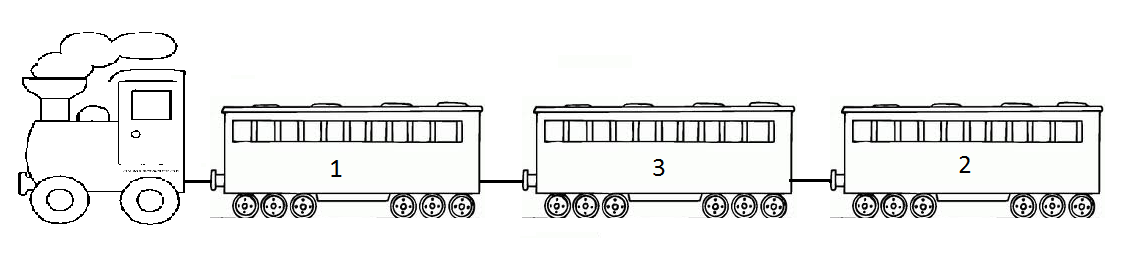
\includegraphics[width=0.50\textwidth]{Tren_Ej1_1.png}
	\\Ejemplo 1.1: Tren desordenado.
\end{center}

\begin{center}
	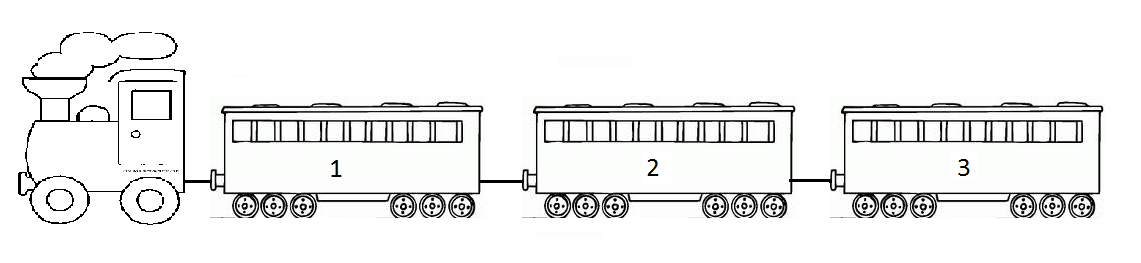
\includegraphics[width=0.50\textwidth]{Tren_Ej1_2.png}
	\\Ejemplo 1.2: Tren ordenado.
\end{center}

En el segundo ejemplo se presenta un tren de 4 vagones:

\begin{center}
	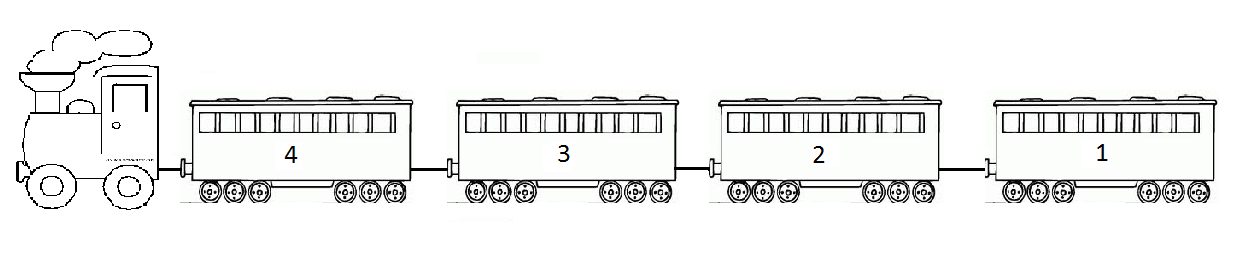
\includegraphics[width=0.50\textwidth]{Tren_Ej2_1.png}
	\\Ejemplo 2.1: Tren desordenado.
\end{center}

\begin{center}
	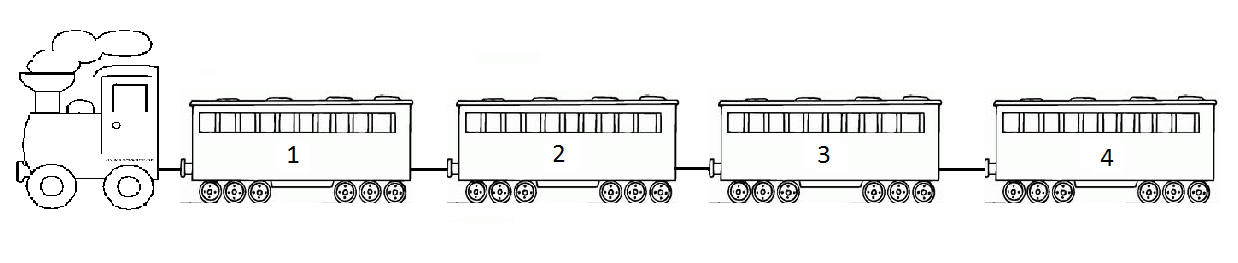
\includegraphics[width=0.50\textwidth]{Tren_Ej2_7.png}
	\\Ejemplo 2.2: Tren ordenado.
\end{center}

\section{Definici�n del problema}
Este problema busca ordenar una lista de trenes, cada uno marcado con un n�mero, en forma ascendente, es decir de menor a mayor. 
\subsection{Entrada}
En la primera linea entra un valor que determina el n�mero casos que habr�n.
\\Seguido a esto entran cada uno de los casos de prueba en dos partes; la primera consta de un n�mero que indica la longitud del tren (Menor que 50), y finalmente entran todos los vagones en el orden actual.
\subsection{Salida}
Imprime la siguiente frase: 
\begin{center}
\textsl{Optimal train swapping takes X swaps.}
\end {center}
donde X es un entero que indica la cantidad de pasos que tuvo que hacer para organizar el vector.
\section{Modelamiento matem�tico}
Se sabe que el tren est� organizado si:
\[
Ordenado\equiv(\forall i,j | 0<i<j<50 : V_{i+1}=V_{j})
\]
Sobre este problema se podr�a extender un �rbol de posibilidades, el cual tendr�a todas las posibles permutaciones que habr�an, donde una de estas es la que satisface la condici�n de salida: Tener todos los vagones ordenados.
\\Analizando el ejemplo 1, existen 6 posibles permutaciones de las cuales s�lo servir�a 1.
\section{Planteamiento de la Soluci�n}
Aunque abrir un �rbol de posibilidades permite analizar mejor el problema, no es la mejor soluci�n, debido a que es poco eficiente; es por ello que existen varios algoritmos de ordenamiento, los cuales permiten organizar una lista en una secuencia dada. Para este problema se usa el algoritmo burbuja.
\\Ordenamiento por Burbuja: Consiste en organizar el vector revisando cada elemento de la lista y compar�ndolo con el siguiente, de esta forma si est�n en el orden equivocado se deben intercambiar. 
\\Aplicando esto al ejemplo 2 se tendr�a lo siguiente:

\begin{center}
	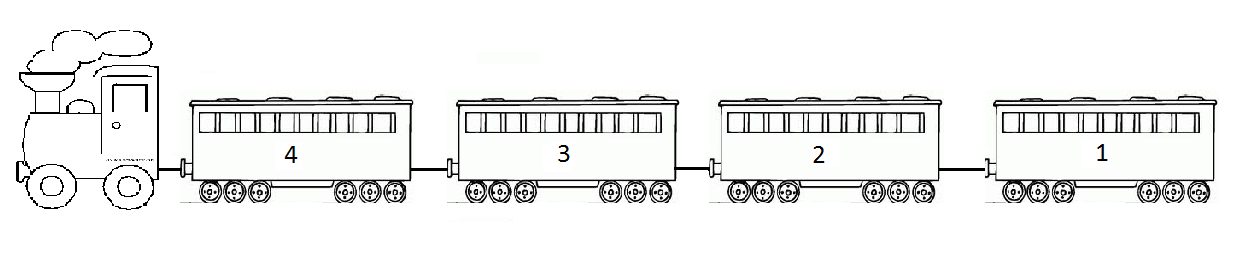
\includegraphics[width=0.50\textwidth]{Tren_Ej2_1.png}
	\\Ejemplo 2.3: Tren Original.
\end{center}

\begin{center}
	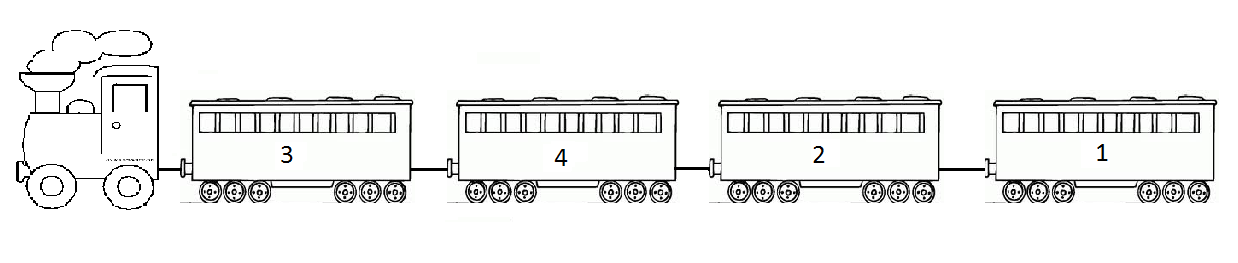
\includegraphics[width=0.50\textwidth]{Tren_Ej2_2.png}
	\\Ejemplo 2.4: Paso 1.
\end{center}

\begin{center}
	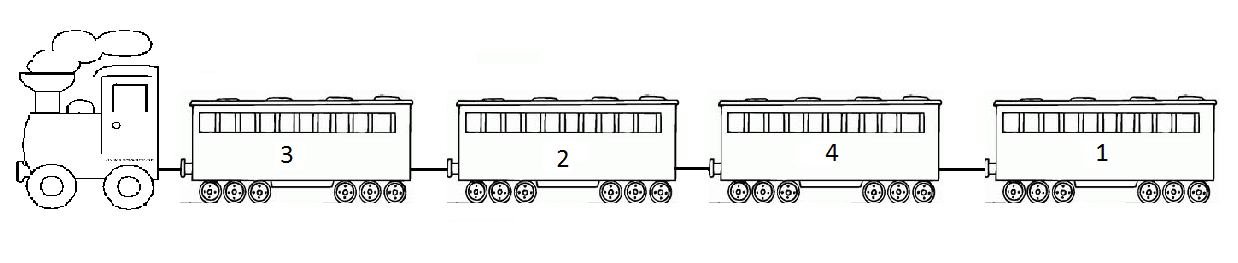
\includegraphics[width=0.50\textwidth]{Tren_Ej2_3.png}
	\\Ejemplo 2.5: Paso 2.
\end{center}

\begin{center}
	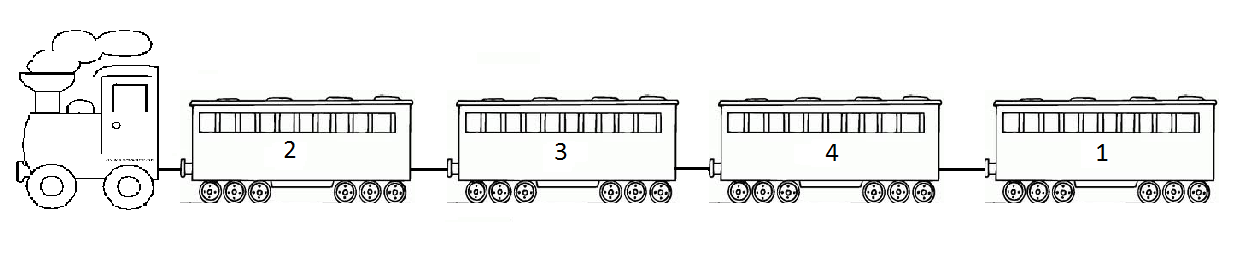
\includegraphics[width=0.50\textwidth]{Tren_Ej2_4.png}
	\\Ejemplo 2.6: Paso 3.
\end{center}

\begin{center}
	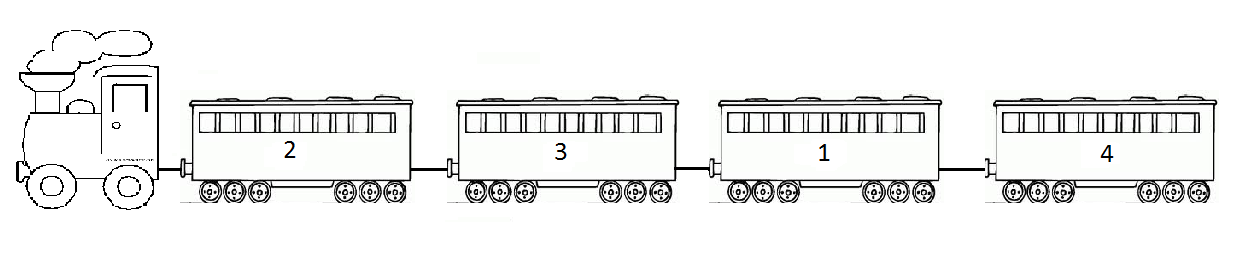
\includegraphics[width=0.50\textwidth]{Tren_Ej2_5.png}
	\\Ejemplo 2.7: Paso 4.
\end{center}

\begin{center}
	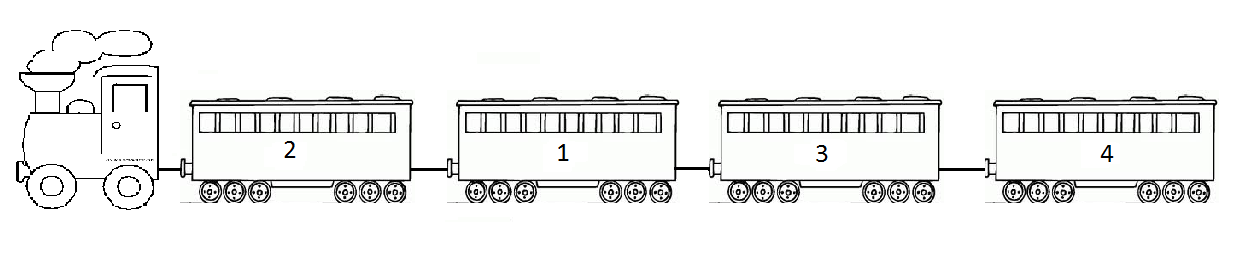
\includegraphics[width=0.50\textwidth]{Tren_Ej2_6.png}
	\\Ejemplo 2.8: Paso 5.
\end{center}

\begin{center}
	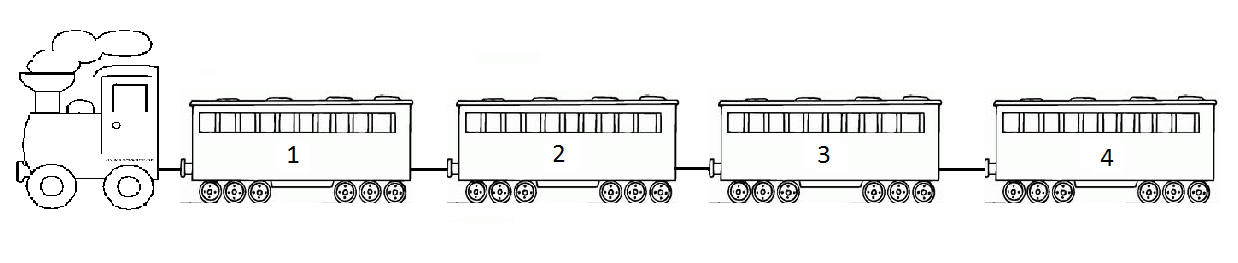
\includegraphics[width=0.50\textwidth]{Tren_Ej2_7.png}
	\\Ejemplo 2.9: Paso 6.
\end{center}
 
\section{Conclusiones}
\begin{enumerate}
	\item Conocer los algoritmos de ordenamiento es importante para optimizar algunos otros algoritmos como los de b�squeda y fusi�n; ya que estos pueden requerir listas ordenadas para tener una ejecuci�n r�pida.
	\item El m�todo de ordenamiento burbuja es el algoritmo de ordenamiento m�s usado en los lenguajes de programaci�n.
\end{enumerate}\end{document}